\section*{Finance implications in training machine learning models}
Another validation technique we considered is to invert the direction of the time dimensions, therefore doing backward forecasting. This can be seen as a form of data augmentation, to have more data to train with. This works for some kind of time series data, for example river levels, but it has been proved not suitable for financial returns data \cite{FLANAGAN20161689} \cite{ramsey1996time}. 
Deterministic tests exist able to distinguish financial times series between originals and the one inverted temporally.  
This can be explained by analysing volatility, that is usually constant, aside from rare moments of volatility spikes. After those spikes, volatility descends, but more slowly than it had risen. By inverting returns, this would produce a slow increase and a sudden fall. 
Another test is based on the leverage effect. There is negative correlation between current returns and future volatility. Future volatility will increase much more from a current negative returns than from a current positive return. Because a negative returns is seen from investors as an increase of risk, while a positive return not. 
But this correlation is not existent between past volatility and future returns, this is a factor exploited by a test for distinguishing original and flipped financial returns time series. 

\section*{PyPortfolioOpt}

PyPortfolioOpt is a Python library that implements several portfolio optimization method and visualizations. It currently supports efficient frontier techniques and Black-Litterman allocation, as well as more recent advances in the area such as shrinkage and Hierarchical Risk Parity, as well as some innovative experimental features such as exponentially-weighted covariance matrices\cite{Martin2021}. 
The library emphasize modularity: users are able to come up with their alternative models and data and feed them into the optimizer.

\hfill \break

Optimization is made starting from expected returns and assets covariance matrix. The library itself implements several methods for forecasting expected returns from simple historical mean, to exponentially weighted mean and capital asset model \cite{investmentscience}. 
The covariance matrix can be obtained also from historical prices by a directed method or exponentially weighted.
In this review we will show only 2 methods of optimization offered by PyPortfolioOpt, EfficientFrontier and EfficientSemivariance. Figure \ref{fig:pyportfolioopt_methods} 
is a graphic summary of the functions offered by the two classes. Some methods are common in both classes, others only of one of them.

\begin{figure}
    \centering
    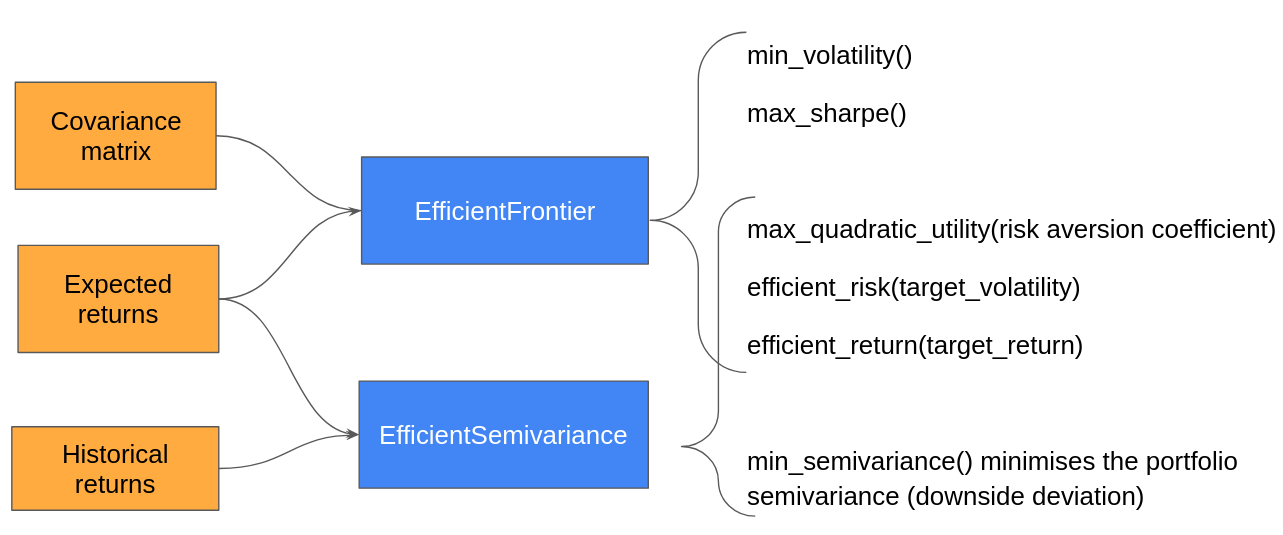
\includegraphics[width=\textwidth]{Appendix/pyportfolioopt_methods.png}
    \caption[PyPortfolioOpt optimization functions]{Optimization function offered by EfficientFrontier and EfficientFrontier, PyPortfolioOpt Python classes}
    \label{fig:pyportfolioopt_methods}
\end{figure}

EfficientFrontier only required the assets Covariance matrix and the Expected returns, while EfficientSemivariance computes internally the Semivariance matrix so requires the historical return and the expected returns.

The \texttt{min\_volatility()}, \texttt{max\_sharpe()} are straighforward and does not require any parameter. \texttt{efficient\_risk} and \texttt{efficient\_return} takes respectively a target volatility and target return. \texttt{min\_semivariance()} minimize the portfolio semivariance as explained in chapter \ref{CH:theoryFI}. \texttt{max\_quadratic\_utility} maximize the function: 

$$ w^T \mu - \frac{\delta}{2} w^T \Sigma w $$ 

It takes as argument a risk aversion coefficient $\delta$ that must be a positive float.  

PyPortfolioOpt also offers several plotting methods that help the understanding of mean-variance theory. The following figures are created from the strategy assets returns that have been used throughout this work. 

Figure \ref{fig:efficient_frontier_assets} is a mean-variance diagram showing the 4 assets strategy on SP500, NASDAQ, EUROSTOXX50, NIKKEI225 and the efficient frontier position for a portfolio built with those assets.

\begin{figure}[h]
    \centering
    \subfloat[\centering without shorting]{{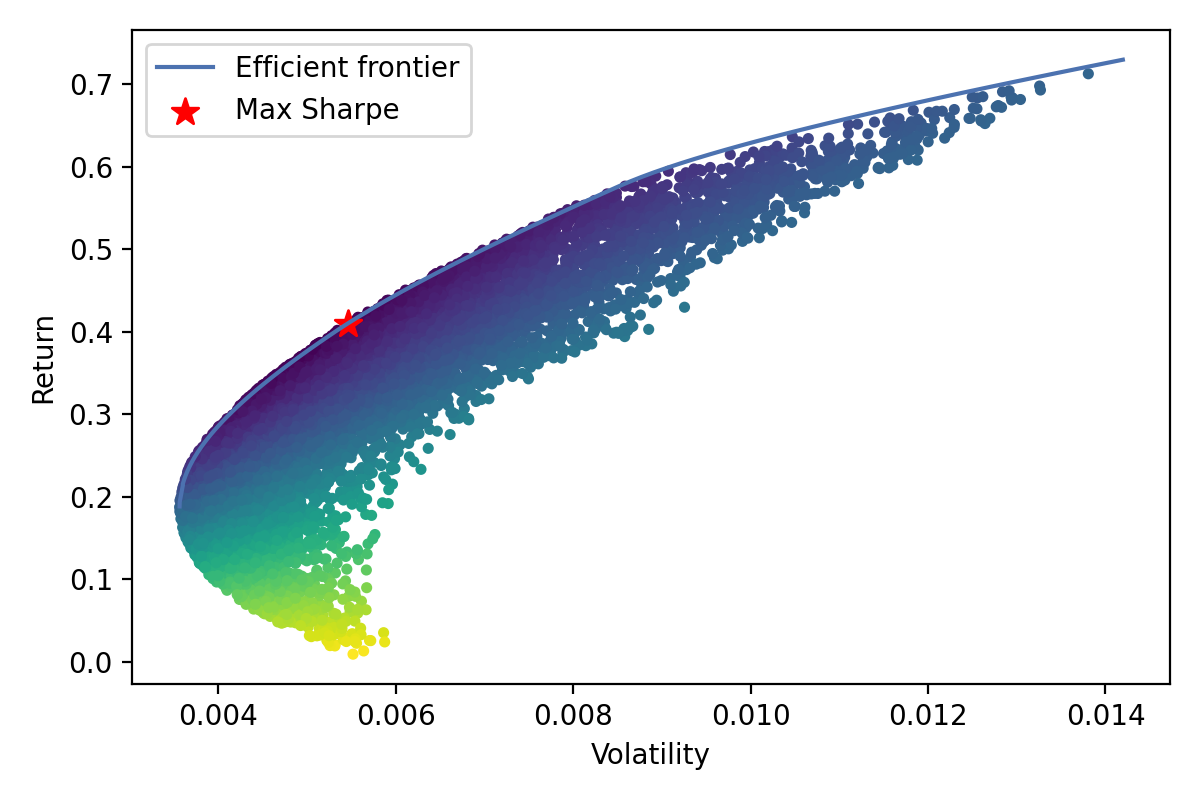
\includegraphics[width=10cm]{Appendix/ef_portfolios.png} }}%
    \qquad
    \subfloat[\centering with shorting ]{{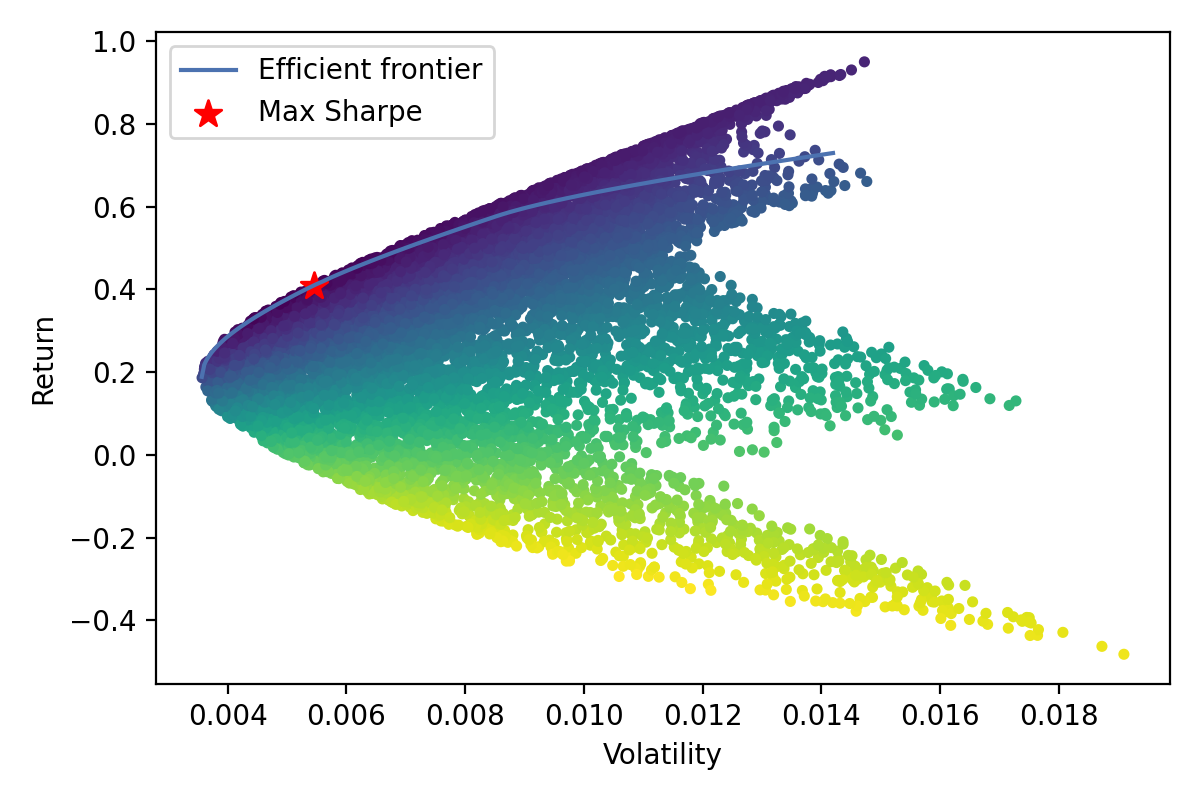
\includegraphics[width=10cm]{Appendix/ef_portfolios_short.png} }}%
    \caption{Mean-Variance diagram: random portfolios}%
    \label{fig:random_portoflios}%
\end{figure}


The coloured dots in figure \ref{fig:random_portoflios} represents different, not necessary optimal, portfolios built starting from those 4 assets, respectively if short selling is allowed or not. These coloured dots are contained in the  feasible region. The star dot is the position of the portfolio that maximize the Sharpe ratio.


